% Example figure with footnote
\begin{figure}[htb]
    \centering
    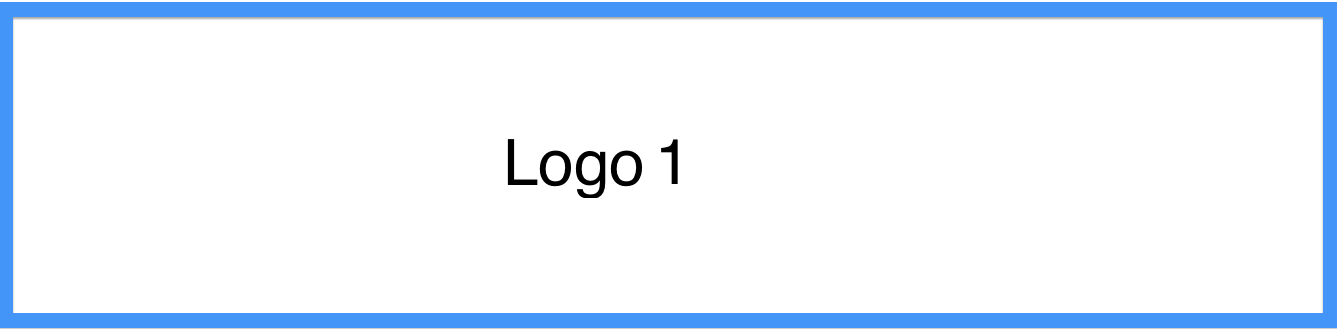
\includegraphics[width=0.4\textwidth,angle=45]{figures/appendix/appendix1.png}
    \caption[Figure example one with footnote]{Figure example one wit footnote\footnotemark}
    \label{fig:exampleone}
\end{figure}
\footnotetext{Figure example one with footnote}

% Example figure
\begin{figure}[htb]
    \centering
    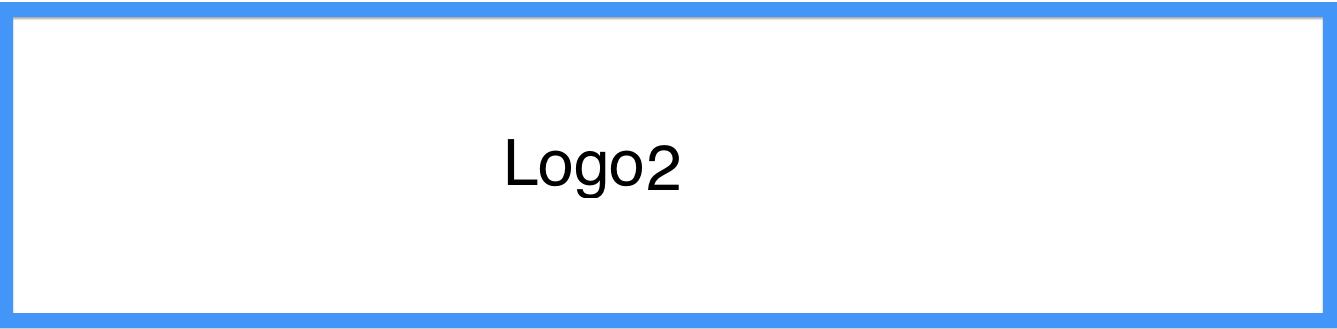
\includegraphics[width=0.3\textwidth,angle=0]{figures/appendix/appendix2.png}
    \caption[Figure example two]{Figure example two}
    \label{fig:exampletwo}
\end{figure}

Refer to figure~\ref{fig:exampleone} on page~\pageref{fig:exampleone}.


% Example table
\begin{table}[htbp]
    \centering
    \begin{tabular}{ | l | c | }
        \hline
        Headline 1 & Headline 2 \\ \hline \hline
        Info 1 & Info 2 \\ \hline
        Info 3 & Info 4 \\ \hline
        \hline
        \multicolumn{2}{|c|}{Info in one row} \\
        \hline
  \end{tabular}
    \caption[Table example]{Table example}
    \label{tab:example}
\end{table}


% Listing example: XML
% Set language to xml
\lstset{language=xml}
\begin{lstlisting}[frame=htrbl, caption={The file {\normalfont \ttfamily  data-config.xml} is an example for XML in LaTeX}, label={lst:dataconfigxml}]
<dataConfig>
  <dataSource type="JdbcDataSource" 
              driver="com.mysql.jdbc.Driver"
              url="jdbc:mysql://localhost/bms_db"
              user="root" 
              password=""/>
  <document>
    <entity name="id"
        query="select id, htmlBody, sentDate, sentFrom, subject, textBody
        from mail">
    <field column="id" name="id"/>
    <field column="htmlBody" name="text"/>
    <field column="sentDate" name="sentDate"/>
    <field column="sentFrom" name="sentFrom"/>
    <field column="subject"  name="subject"/>
    <field column="textBody" name="text"/>
    </entity>
  </document>
</dataConfig>
\end{lstlisting}

% Listing example: Java
% Set language to java (Java is default in this document)
\lstset{language=java}
\begin{lstlisting}[frame=htrbl, caption={Listing displays Java code}, label={lst:javacode}]
/* generate TagCloud */
Cloud cloud = new Cloud();
cloud.setMaxWeight(_maxSizeOfText);
cloud.setMinWeight(_minSizeOfText);
cloud.setTagCase(Case.LOWER);
	    
/* evaluate context and find additional stopwords */
String query = getContextQuery(_context);
List<String> contextStoplist = new ArrayList<String>();
contextStoplist = getStopwordsFromDB(query);
	    
/* append context stoplist */
while(contextStoplist != null && !contextStoplist.isEmpty())
  _stoplist.add(contextStoplist.remove(0));
	    
/* add cloud filters */
if (_stoplist != null) {
  DictionaryFilter df = new DictionaryFilter(_stoplist);
  cloud.addInputFilter(df);
}
/* remove empty tags */
NonNullFilter<Tag> nnf = new NonNullFilter<Tag>();
cloud.addInputFilter(nnf);

/* set minimum tag length */
MinLengthFilter mlf = new MinLengthFilter(_minTagLength);
cloud.addInputFilter(mlf);

/* add taglist to tagcloud */
cloud.addText(_taglist);

/* set number of shown tags */	    
cloud.setMaxTagsToDisplay(_tagsToDisplay);
\end{lstlisting}


% Example for equations
Die Zuordnung aller möglichen Werte, welche eine Zufallsvariable annehmen kann, nennt man \emph{Verteilungsfunktion} von $X$.

\begin{quotation}
Die Funktion F: $\mathbb{R} \rightarrow$ [0,1] mit $F(t) = P (X \le t)$ heißt Verteilungsfunktion von $X$.\footnote{Mustermann, vgl.~\cite{mm2009}~[p.55]}
\end{quotation}

Für eine stetige Zufallsvariable $X: \Omega \rightarrow \mathbb{R}$ heißt eine integrierbare, nicht negative reelle Funktion $w: \mathbb{R} \rightarrow \mathbb{R}$ mit $F(x) = P(X \le x) = \int_{-\infty}^{x} w(t)dt$ die \emph{Dichte} oder \emph{Wahrscheinlichkeitsdichte} der Zufallsvariablen $X$.\footnote{Mustermann, vgl.~\cite{mf2005}~[p.56]}
